% Created 2017-03-01 Wed 20:38
\documentclass[10pt]{article}
\usepackage[utf8]{inputenc}
\usepackage[T1]{fontenc}
\usepackage{fixltx2e}
\usepackage{graphicx}
\usepackage{longtable}
\usepackage{float}
\usepackage{wrapfig}
\usepackage{rotating}
\usepackage[normalem]{ulem}
\usepackage{amsmath}
\usepackage{textcomp}
\usepackage{marvosym}
\usepackage{wasysym}
\usepackage{amssymb}
\tolerance=1000
\usepackage{natbib}
\usepackage[linktocpage,pdfstartview=FitH,colorlinks,
linkcolor=blue,anchorcolor=blue,
citecolor=blue,filecolor=blue,menucolor=blue,urlcolor=blue]{hyperref}
\usepackage[margin=2cm]{geometry}
\pagenumbering{gobble}
\usepackage{wrapfig}
\usepackage{multicol}
\setlength\columnsep{20pt}
\author{Alejandro Rodríguez Salamanca: r0650814@student.kuleuven.be}
\date{}
\title{Artificial Neural Networks: Exercise session 1}
\begin{document}

\maketitle
\begin{multicols}{2}

\section*{Exercise 1}

For this exercise, three different algorithms has been compared against Gradient Descent:
Levenberg-Marquardt, BFGS Quasi-Newton and Polak-Ribiere conjugate gradient.
The data has been optained in different phases of the training process, after 50 epochs,
300 epochs and 1000 epochs, to determine not only which algorithm fits the function more precisely, 
but also faster.

The function to approximate is \texttt{y = sin(x)} with points between 0 and 4$\pi$.

\subsection*{Comparison of algorithms}

\begin{itemize}
\item Gradient Descent vs. Levenberg-Marquardt

As we can see in the plots, \textit{Levenberg-Marquardt} outperforms \textit{Gradient Descent} since the begining.
At 50 epochs, LM has perfectly fitted the function, while GD is far from that even with 1000 epochs. As we have studied in class, GD is more prone to get stuck in a local minima. Anyhow, the performance of LM is surprisingly good.

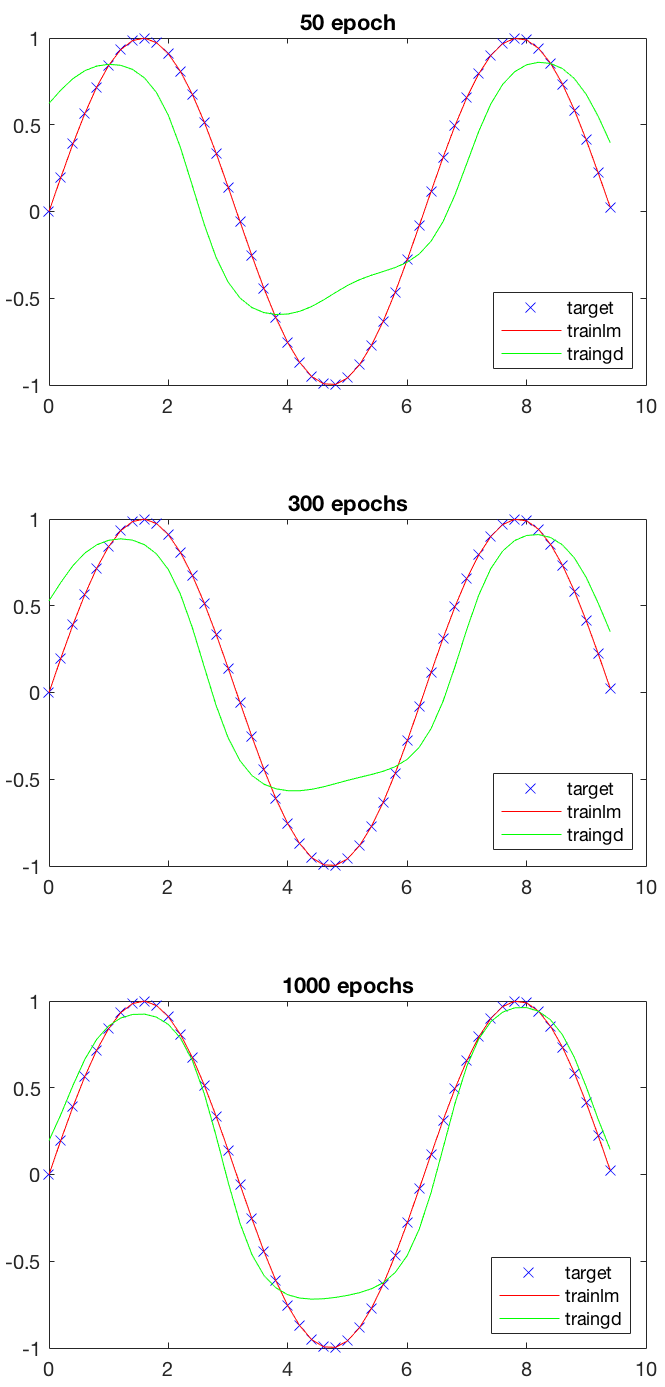
\includegraphics[width=.65\linewidth]{img/vsLMep}

\item Gradient Descent vs. BFGS Quasi-Newton

\textit{Quasi-Newton} outperforms sifnifically \textit{Gradient Descent}, but the results obtained are not as good
as with LM. At 50 epochs it can be seen that QN has approximated the function fairly well, but it does no have the precission shown by LM. At 300 epochs, it fits the function \texttt{y = sin(x)}.

\item Gradient Descent vs. Polak-Ribiere conjugate gradient

\textit{Polak-Ribiere}'s results are simillar to the ones obtained with QN. It outperfoms significally GD since the very first iteration. At 50 epochs the aproximation is really close to the function \texttt{y = sin(x)}, and once reached the epoch 300, that aproximation fits the function perfectly.

On the other hand, the performance of GD is similar to the one shown with the previous methods: at 1000 epochs,
the aproximation is far from fitting the function \texttt{y}.

\end{itemize}

\subsection*{Learning from noisy data: Generalization}

The noise to the data has been added using

\begin{verbatim}
 noisy_y = y + 0.3 * rand(1, length(y));
\end{verbatim}

This add noise to the function \texttt{y} with an amplitude of 0.3.

Now, the points does not follow a perfect \texttt{sin} function, so the algorithm should find more difficult to
guess the underlying function of the dataset.

The three algorithms used performs in a similar way. At 50 epochs, the aproximation is really close to a \texttt{sin} function, and at 300 epochs, they have already guessed the underlying function.

It's important to look at the performance of the \textit{Gradient Descent}. When noise is added to the function,
it can be seen that this method is able to find a better aproximation that in the previous section.

Now, it's time to compare the performance of the algorithms when there is noise in the data or not, in terms of epochs. Note that the training of the Neural Network stops when the maximun number of epochs is reached, or when the Mean Squared error is minimum.

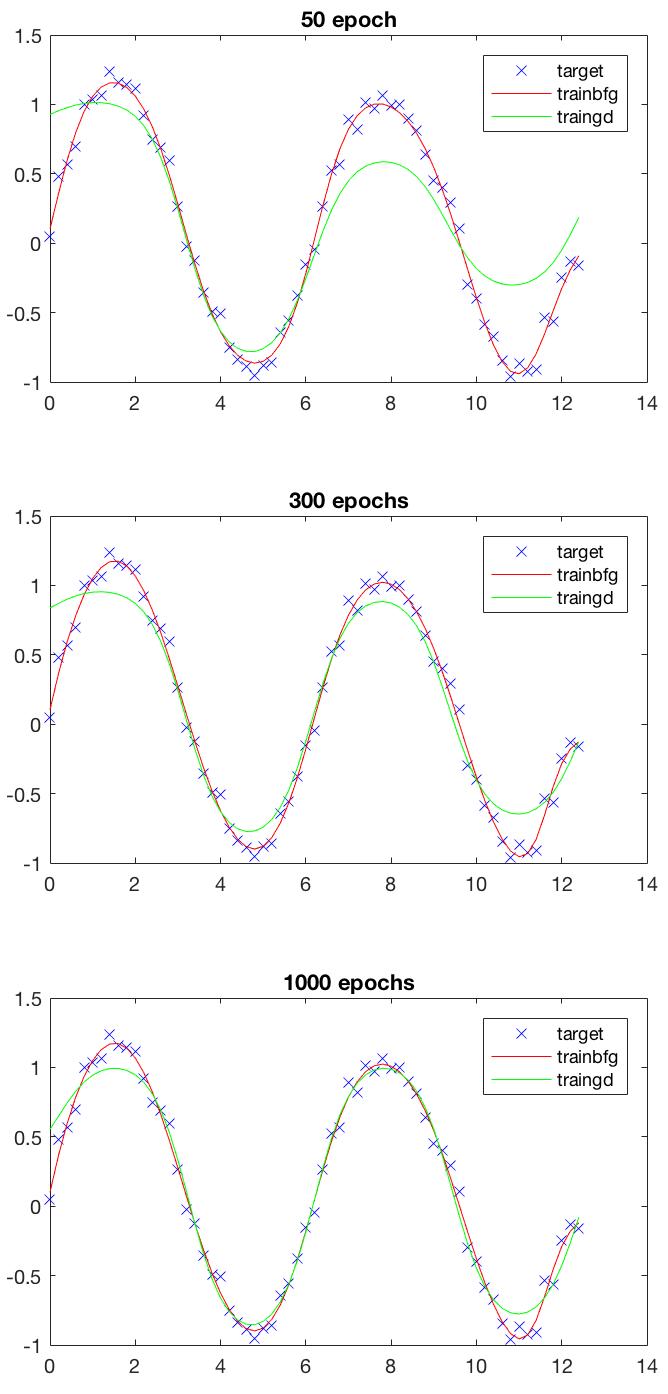
\includegraphics[width=.65\linewidth]{img/vsBFGnoisyEp}

The two plots show the performance using \textit{Levenberg-Marquardt} without noise and with noise.
As we should expect, the error is much lower when there is no noise in the data, showing a value of $10^{-8}$. Actually, an error of this magnitude can be due to the precission of floating point numbers.

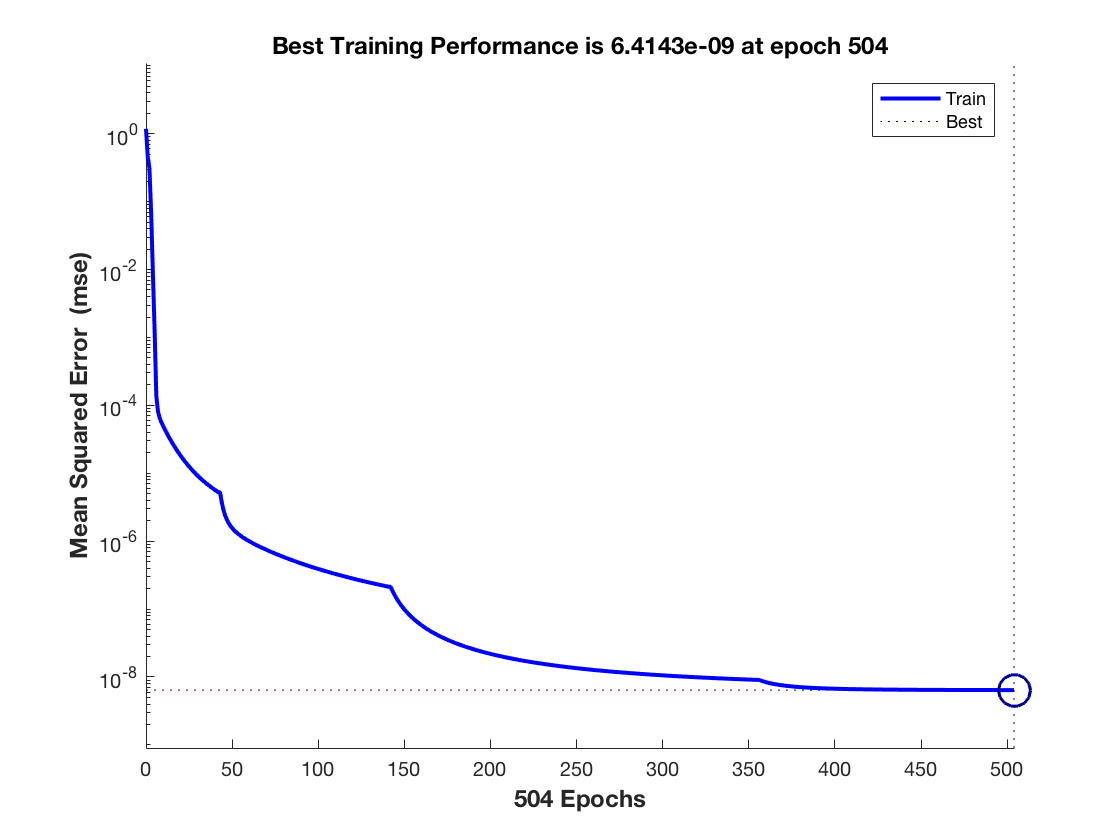
\includegraphics[width=.7\linewidth]{img/perfLM}

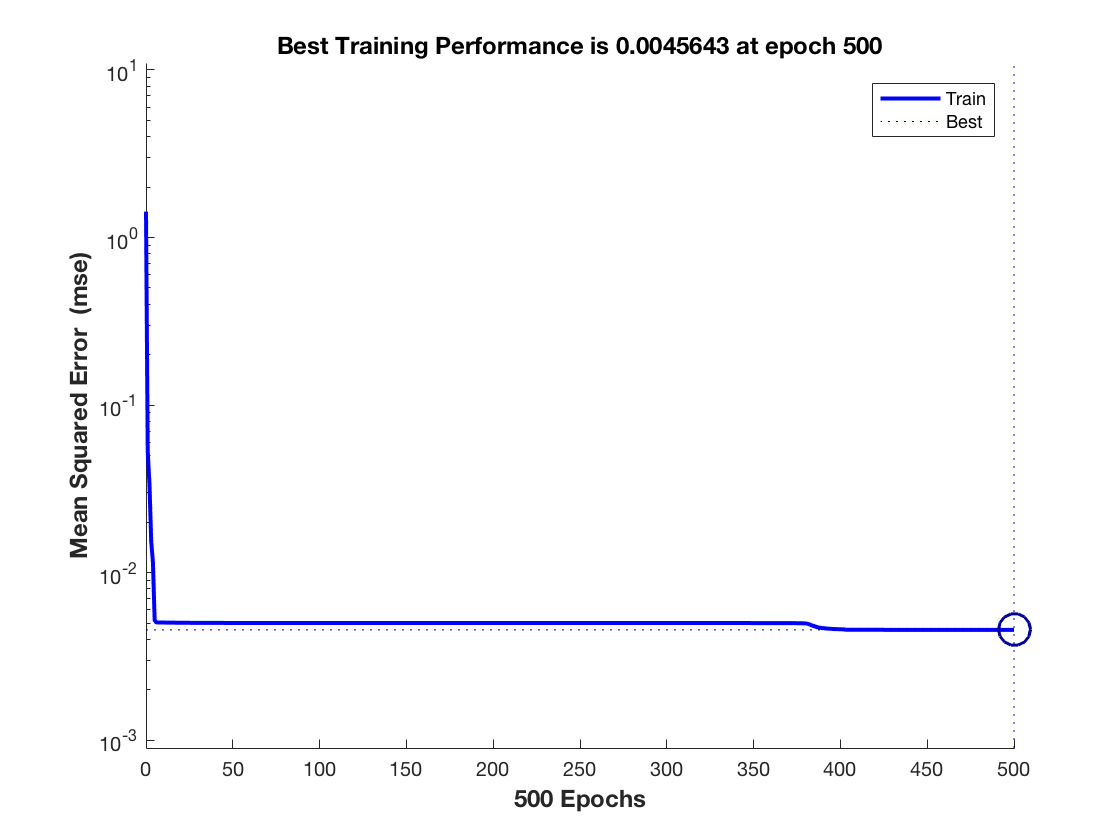
\includegraphics[width=.7\linewidth]{img/perfLMnoisy}

\section*{Exercise 2}
For this second exercise, the results obtained with \texttt{trainbr} where astounding. For this reason, the number of points were doubled and the amplitued of the noise where changed to 1. 

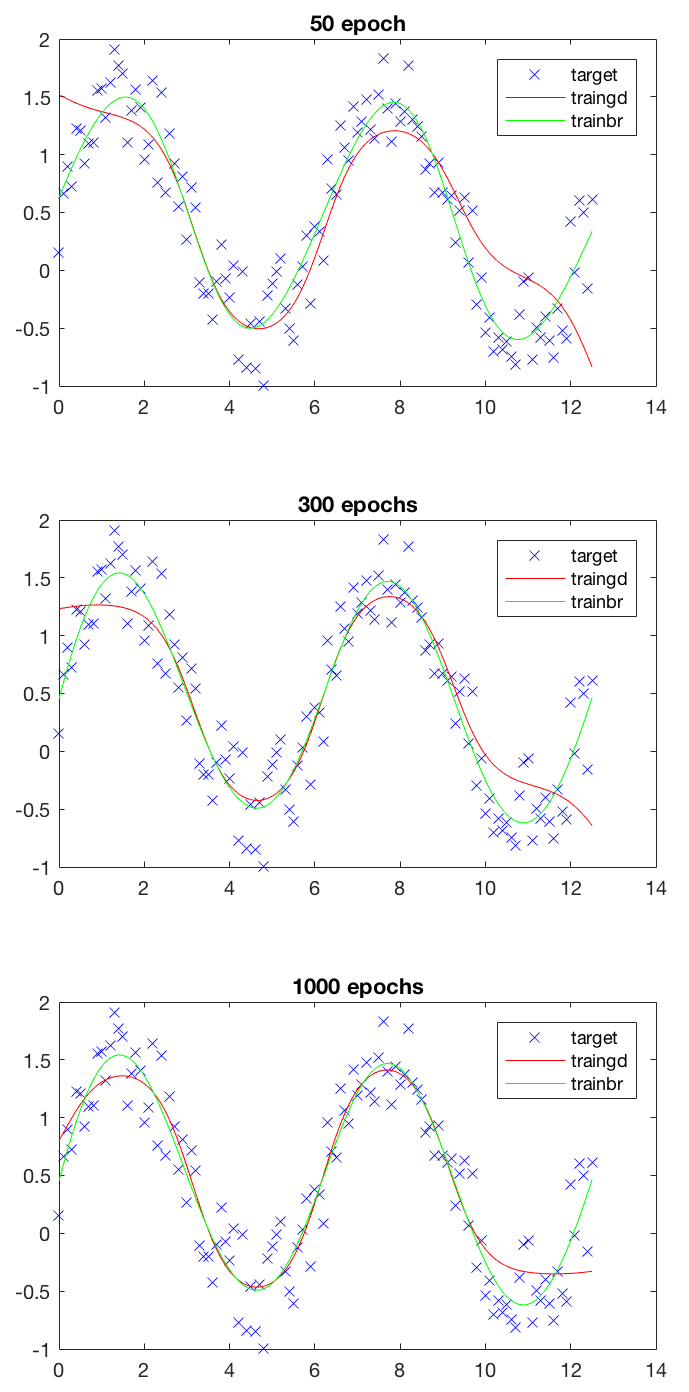
\includegraphics[width=.65\linewidth]{img/vsBRnoisyEp}

It can be seen in the plot that even after adding more noise to the data, at 50 epochs the algorithm is capable of 
aproximate the function. Actually, it can be seen in the following plot that it only needs 31 epochs to minimize the mean square error.

This means that this algorithms outperforms all the algorithms studied in the previous exercise.

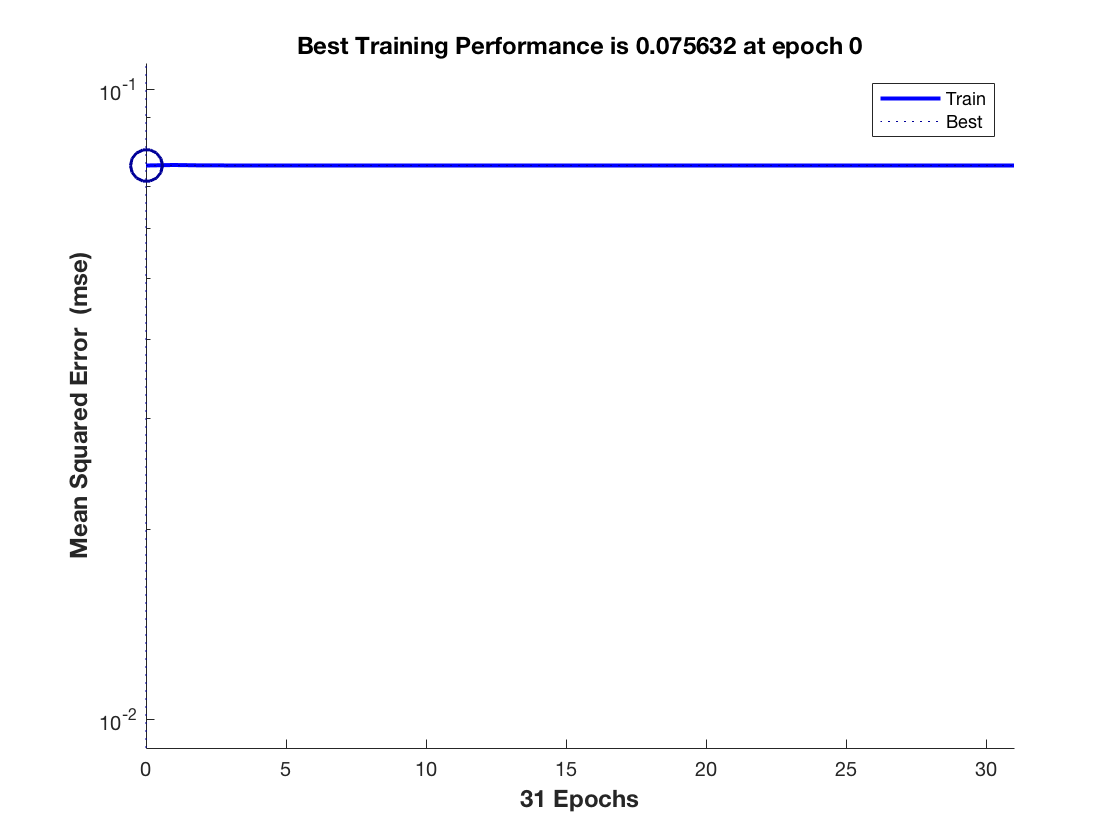
\includegraphics[width=.7\linewidth]{img/errBR}


\end{multicols}
\end{document}